\documentclass{article}
% \usepackage[utf8]{inputenc}
\usepackage{tikz}

\tikzstyle{n}=[rectangle, draw=black, fill=red, thick, minimum width=7cm, minimum height=7cm, align= center]

\begin{document}

\vskip40pt
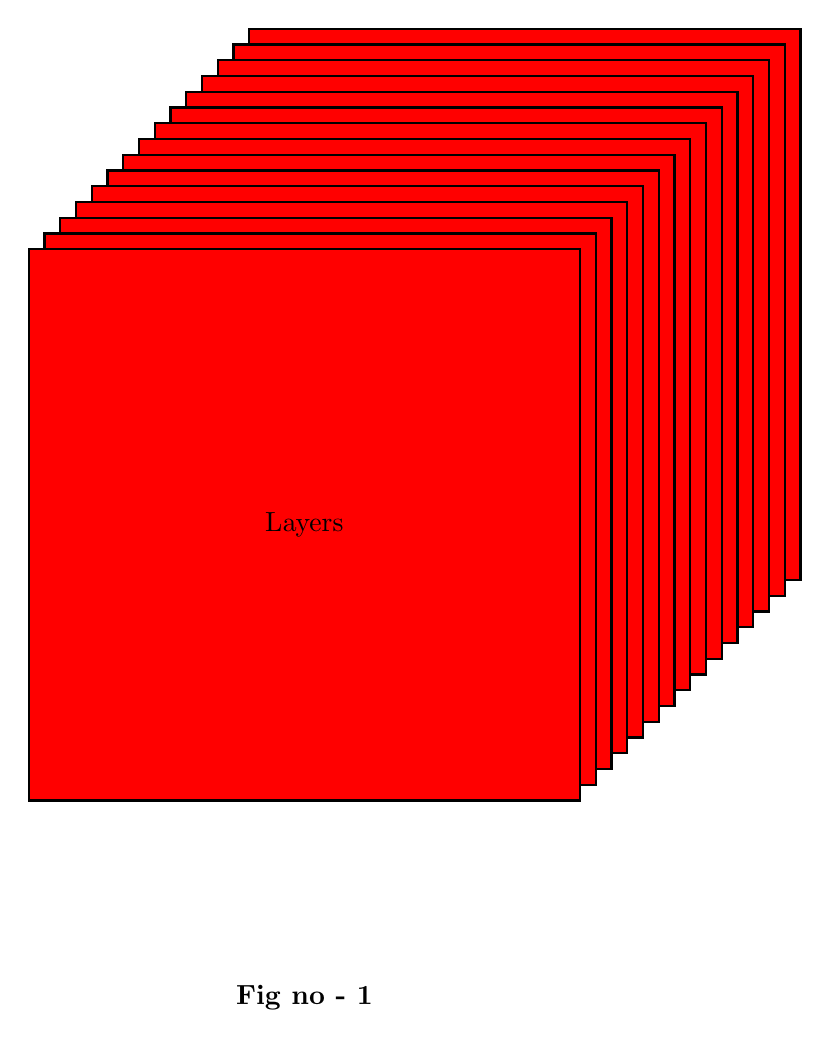
\begin{tikzpicture}
      \foreach \x in {1,...,15}
     {
            \node[n] (1) at (5-0.2*\x, 5-0.2*\x) {Layers};
     }
     \node(1) at (2,-4){\textbf{Fig no - 1}};
\end{tikzpicture}



\newpage


\tikzstyle{big}=[circle, draw=white, fill=blue!90, minimum size=3cm, text=white]
\tikzstyle{b}=[rectangle, draw=white, maximum size=3cm, align=center ]
\tikzstyle{sm}=[circle, draw=black, very thick, minimum size=1cm, align=center]
\tikzstyle{arr}=[->,>=stealth, very thick]
    
\begin{tikzpicture}
\node[sm] (1) {$x0=1$};
\node[sm,below=2cm](2)  at (1){x1};
\node[sm,below=2cm](3)  at (2){x2};
\node[big,below=1cm, right=3cm](4)  at (2){z   f};
\node[left=1cm,above=0.5cm,very thick](inp) at(1){Inputs};
\node[below=1.5cm, very thick](a) at (3){...};
\node(x) at (3,-8){\textbf{Fig no - 2}};
\node[above=1.5cm, right=0.5cm](ab) at (4){};
\node[below=1.5cm,right=0.5cm](be) at (4){};
\node[right=5cm] (5) at (4){};
\node[right=3cm,below=0.5cm, very thick](6)at (4){\textbf{Output}};
\node[b, below=2cm, left=0.5 cm](l) at (4){Linear function};
\node[b, below=2cm, right=0.5cm](r) at (4){Activation function};

\draw[arr] (inp.south) -- (1.west);
\draw[arr] (inp.south) -- (2.west);
\draw[arr] (1.east) -- node[above]{b} (4.west) ;
\draw[arr] (2.east) -- node[above]{w1}(4.west) ;
\draw[arr] (3.east) -- node[above]{w2} (4.west) ;
\draw[arr](4.east)--node[above]{y}(5);
\draw[arr](l)--(4);
\draw[arr](r)--(4);
% \draw[dashed,color] (ab)|(be);

\end{tikzpicture}

\end{document}